\documentclass[border=12pt]{standalone}
\usepackage{tikz}
\usetikzlibrary{shapes.geometric, arrows.meta, positioning, calc, fit, backgrounds}
\usepackage{fontspec}
\usepackage{amsmath,amssymb}
\setmainfont{DejaVu Sans}

\begin{document}
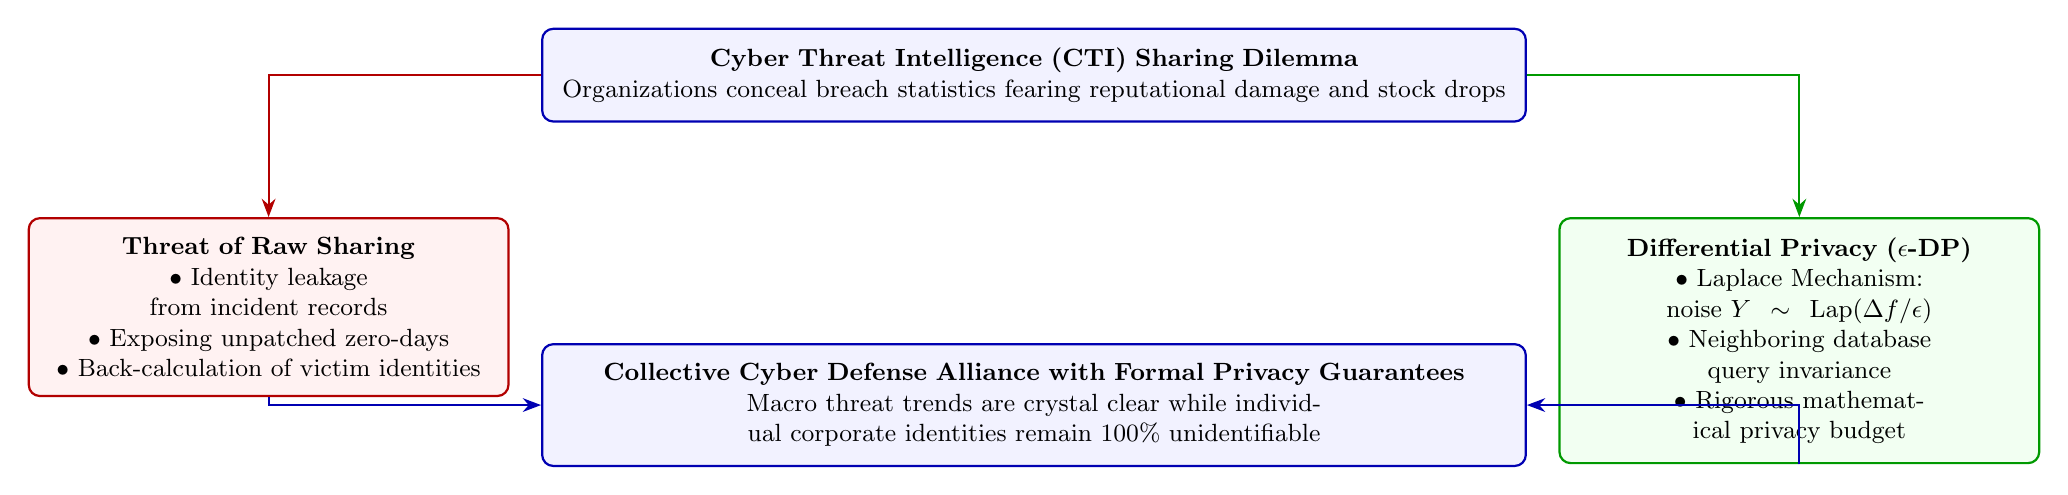
\begin{tikzpicture}[
    font=\small,
    >=Stealth,
    node distance=1.2cm,
    block/.style={rectangle, draw=blue!70!black, fill=blue!5, rounded corners=4pt, thick, align=center, inner sep=7pt},
    alertblock/.style={rectangle, draw=red!70!black, fill=red!5, rounded corners=4pt, thick, align=center, inner sep=7pt},
    greenblock/.style={rectangle, draw=green!60!black, fill=green!5, rounded corners=4pt, thick, align=center, inner sep=7pt},
    amberblock/.style={rectangle, draw=orange!80!black, fill=orange!5, rounded corners=4pt, thick, align=center, inner sep=7pt}
]

\node[block, text width=12cm] (top) {\textbf{Cyber Threat Intelligence (CTI) Sharing Dilemma}\\Organizations conceal breach statistics fearing reputational damage and stock drops};

\node[alertblock, below left=1.2cm and 0.4cm of top, text width=5.6cm] (dilemma) {\textbf{Threat of Raw Sharing}\\$\bullet$ Identity leakage from incident records\\$\bullet$ Exposing unpatched zero-days\\$\bullet$ Back-calculation of victim identities};

\node[greenblock, below right=1.2cm and 0.4cm of top, text width=5.6cm] (dp) {\textbf{Differential Privacy ($\epsilon$-DP)}\\$\bullet$ Laplace Mechanism: noise $Y \sim \text{Lap}(\Delta f / \epsilon)$\\$\bullet$ Neighboring database query invariance\\$\bullet$ Rigorous mathematical privacy budget};

\node[block, below=2.8cm of top, text width=12cm] (bottom) {\textbf{Collective Cyber Defense Alliance with Formal Privacy Guarantees}\\Macro threat trends are crystal clear while individual corporate identities remain 100\% unidentifiable};

\draw[->, thick, red!70!black] (top) -| (dilemma);
\draw[->, thick, green!60!black] (top) -| (dp);
\draw[->, thick, blue!70!black] (dilemma) |- (bottom);
\draw[->, thick, blue!70!black] (dp) |- (bottom);

\end{tikzpicture}
\end{document}
